%%%%%%%%%%%%%%%%%%%%%%%%%%%%%%%%%%%%%%%%%%%%%%%%%%%%%%%%%%%%%%%%%%%%%%%%%%%%%%%%
%2345678901234567890123456789012345678901234567890123456789012345678901234567890
%        1         2         3         4         5         6         7         8

\documentclass[letterpaper, 10 pt, conference]{ieeeconf}  % Comment this line out
                                                          % if you need a4paper
%\documentclass[a4paper, 10pt, conference]{ieeeconf}      % Use this line for a4
                                                          % paper

\IEEEoverridecommandlockouts                              % This command is only
                                                          % needed if you want to
                                                          % use the \thanks command
\overrideIEEEmargins
% See the \addtolength command later in the file to balance the column lengths
% on the last page of the document

\usepackage[utf8]{inputenc}
\usepackage[T1]{fontenc}
\usepackage{graphicx}
\usepackage{wrapfig}
\usepackage[labelformat=empty]{caption}

% The following packages can be found on http:\\www.ctan.org
%\usepackage{graphics} % for pdf, bitmapped graphics files
%\usepackage{epsfig} % for postscript graphics files
%\usepackage{mathptmx} % assumes new font selection scheme installed
%\usepackage{mathptmx} % assumes new font selection scheme installed
%\usepackage{amsmath} % assumes amsmath package installed
%\usepackage{amssymb}  % assumes amsmath package installed

\title{\LARGE \bf
The Exploration in Bitcoin 
}

%\author{ \parbox{3 in}{\centering Huibert Kwakernaak*
%         \thanks{*Use the $\backslash$thanks command to put information here}\\
%         Faculty of Electrical Engineering, Mathematics and Computer Science\\
%         University of Twente\\
%         7500 AE Enschede, The Netherlands\\
%         {\tt\small h.kwakernaak@autsubmit.com}}
%         \hspace*{ 0.5 in}
%         \parbox{3 in}{ \centering Pradeep Misra**
%         \thanks{**The footnote marks may be inserted manually}\\
%        Department of Electrical Engineering \\
%         Wright State University\\
%         Dayton, OH 45435, USA\\
%         {\tt\small pmisra@cs.wright.edu}}
%}

\author{Amy Nguyen % stops a space

}


\begin{document}



\maketitle
\thispagestyle{empty}
\pagestyle{empty}


%%%%%%%%%%%%%%%%%%%%%%%%%%%%%%%%%%%%%%%%%%%%%%%%%%%%%%%%%%%%%%%%%%%%%%%%%%%%%%%%


%%%%%%%%%%%%%%%%%%%%%%%%%%%%%%%%%%%%%%%%%%%%%%%%%%%%%%%%%%%%%%%%%%%%%%%%%%%%%%%%
\section{INTRODUCTION}

Cryptocurrency has been a method of payment for years and is increasing in popularity as time goes by. back in the day, cryptocurrency was seen as an underground currency people use to purchase things through the internet with privacy. Bitcoin is one of the popular forms of cryptocurrency and is in forms of nodes. Those nodes authorize anonymous transactions--which gains the trust of its users. Not only that but the government has no power or control in Bitcoin, the power is nestled in the heart of the system and those that partake in it which could be another reason why people gravitate in investing in crypto. So what exactly is Bitcoin and how does it work? This article will go in depth of how Bitcoin works and why people favor Bitcoin.

\section{HOW BITCOIN WORKS}
\begin{figure}[h!]
  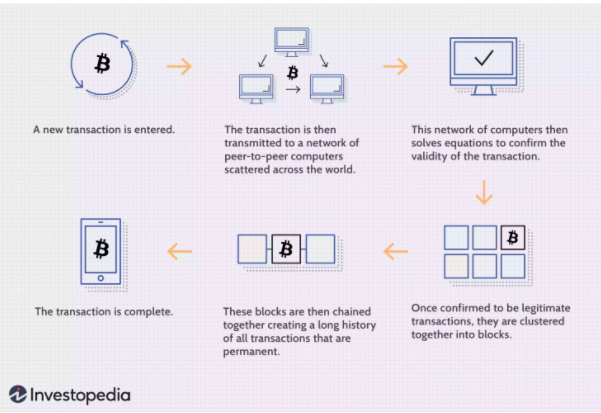
\includegraphics[width=8cm]{process.PNG}
  \caption*{[1]}
\end{figure}
Bitcoin can be obtained either through the purchasing it with real money, exchanging for Bitcoin or from mining. Mining is part of how a transaction gets processed. Let's start at the beginning of how a bitcoin transaction is processed. First a user will make a transaction under a private key. Each user has a public key that is used to identify them and a private key used to verify transactions and exchanges. This is a private key that is unique to the user that no one else knows. The transaction will then be sent to a group of peer-to-peer computers that will then try to solve complex problems to verify the transaction. The validation of the transaction is called "Proof of Work" which means the miner must solve the complex problems with a GPU. As a reward, the person that solves the computational problem is awarded the transaction fees in Bitcoin. After this, the transaction is complete, recorded into a block and then strung together into a block chain of other transactions (think of this as a long receipt). 


\subsection{SECURITY OF BLOCKCHAINS}
\begin{figure}[h!]
  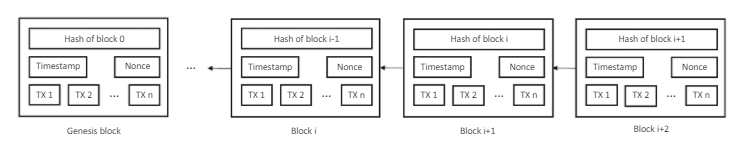
\includegraphics[width=10cm]{blockchain.PNG}
  \caption*{[3]}
\end{figure}
What makes Bitcoin so secure is its blockchain. The maintenance on the blockchain is transparent, immutable, decentralized, and unregulated by the government. This means that what happens to the blockchain is completely shared between users and Bitcoin miners. All the miners share their proof-of-work which contributes to the trust people have in the system powered by and managed by the people themselves \textbf{[2]}. Once a block is added to the chain, it is immutable--meaning that changes cannot be made to the chain. Things can only be added to the chain--not removed nor changed in ensure validity and strengthen the security and fluidity of the chain. So What deters hackers from messing with the blockchain? Well to begin, each block or transaction has a timestamp of the transaction, a hash value of the block preceding it, and a nonce which is a random number to verify its own hash.This is to provide extra security to the blockchain, making it nearly impossible to penetrate. Not only must the transaction be verified by a miner, but it also must be verified by other miners through a consensus mechanism \textbf{[3]}. This builds trust within the miners and the community due to how proactive everyone is. This makes it close to impossible for the blockchain to be hacked. If a hacker wanted to steal money, they would have to alter the entire blockchain. The hacker would have to gain 51\% control over the blockchain and alter the blocks that are consistent to its neighboring blocks.--this is also known as a 51\% attack. Even if the hacker were to alter the blocks in his favor, he must make it so that it is up to date to the current blockchain. The blockchain is constantly growing with new blocks/transactions. So even if the hacker has an altered version of the blockchain, if he doesn't update it to the current chain, the system will always pick the blockchain that contains more blocks. The only time it is possible for a 51\% attack to occur is if a miner has over 50\% control over the blockchain. This makes it easier for hackers to find a vulnerability since most of the chain belongs to one miner. This is why it is important to have the consensus mechanism between the various miners but it doesn't matter as much since it is established that Bitcoin will not allow a miner to have that much control over the blockchain \textbf{[3]}.

\section{HISTORY OF BITCOIN MINING}
\begin{figure}[h!]
  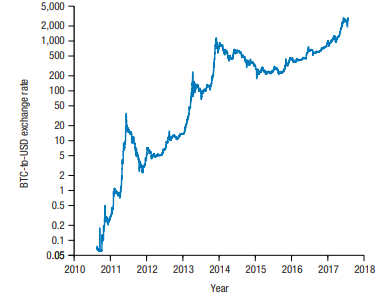
\includegraphics[width=8cm]{exchange.PNG}
  \caption*{[5.a]}
\end{figure}
Bitcoin miners must use computers with powerful GPUs to solve computational problems, competing with other miners for the award of bitcoin. The more powerful the computer is, the higher the probability it is for a miner to win the mining race \textbf{[4]}. However, Bitcoin started out simpler than it is today. People would use old GPUs or their own computers to mine Bitcoin. As you can see from the two figures, as Bitcoin became more popular, the more blocks that are added to the blockchain, resulting more complexity to the computational problems. 
\begin{figure}[h!]
  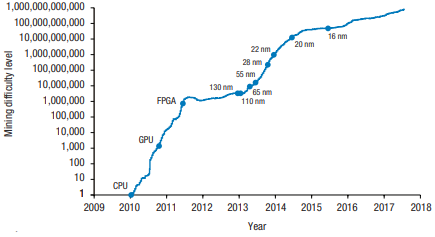
\includegraphics[width=9cm]{diff.PNG}
  \caption*{[5.b]}
\end{figure}
This means miners with normal or average computers will find mining infeasible and have to have the choice to either upgrade to better equipment or give up the race in general. Not only do miners need to spend money on obtaining the hardware to mine Bitcoin, they also need the keep in mind how energy consuming it is for these powerful GPUs to run. 
To gain more probability in earning Bitcoin, people have created mining pools in which are warehouses that consist of technology solely there for mining Bitcoin. There needs to be around the clock maintenance of the systems and Bitcoin miners must keep in mind that there is a lifespan to the GPUs. As time passes, the efficiency of the GPU's ability to solve computational puzzles will decrease contributing to the difficulty to mining for bitcoin. It is a tedious task to make sure one of profiting from mining Bitcoin since it involves constant surveillance to make sure when GPUs are actually spending more resources than they are making. With all of these chances to Bitcoin mining, this makes it not so efficient anymore for a home computer to mine for Bitcoin and mining pools took over \textbf{[5]}. One of the biggest Bitcoin mining pools are located in China which insists of companies such as AntPool, BTC.com, BTC.top, and ViaBTC \textbf{[4]}.

\section{BITCOIN VULNERABILITIES}
Although blockchains may be nearly impossible to hack completely, there has been cases where exchanges themselves have been hacked. Exchanges are company hosted--similar to a brokerage. Users will create a wallet under the company who will hold the money for them to exchange for other cryptocurrencies or to buy cryptocurrency with real money. Although the hack isn't directly related to the blockchain thus not really putting Bitcoin at fault, people still have lost millions worth of their Bitcoin due to hackers that have infiltrated these exchanges in the past. One of the incidents that occurred was the security breach of the Mt. Gox exchange. The hacker managed to tamper with the value of Bitcoin on the Mt. Gox exchange, making it drop to 1\%. Not only did they do that, they also used an auditor's credentials to transfer a large amount of Bitcoins to himself then selling all of it nominally at any given price. Even though the fraudulent changes were reverted after a few minutes, tons of people have lost over 8 million US dollars from this incident. In 2014, Mt. Gow filed for bankruptcy and their CEO was arrested for embezzlement. This is not the only incident that occurred where consumers have lost their money over things out of their power. Another infamous incident that occurred was the Bitfinex hack, where the Bitfinex exchange lost over 72 million US dollars worth of Bitcoin \textbf{[6]}. Hacking incidents like these show that exchanges can lose millions worth of cryptocurrency and also plummet in its value. Due to this, this can place a mistrust and paranoia of consumers in opening up wallets within exchanges. A higher security could be implemented for the exchanges however at the cost of the freedom people have in the peer-to-peer networks which can lose interest in some of the independent Bitcoin miners. 
\begin{figure}[h!]
  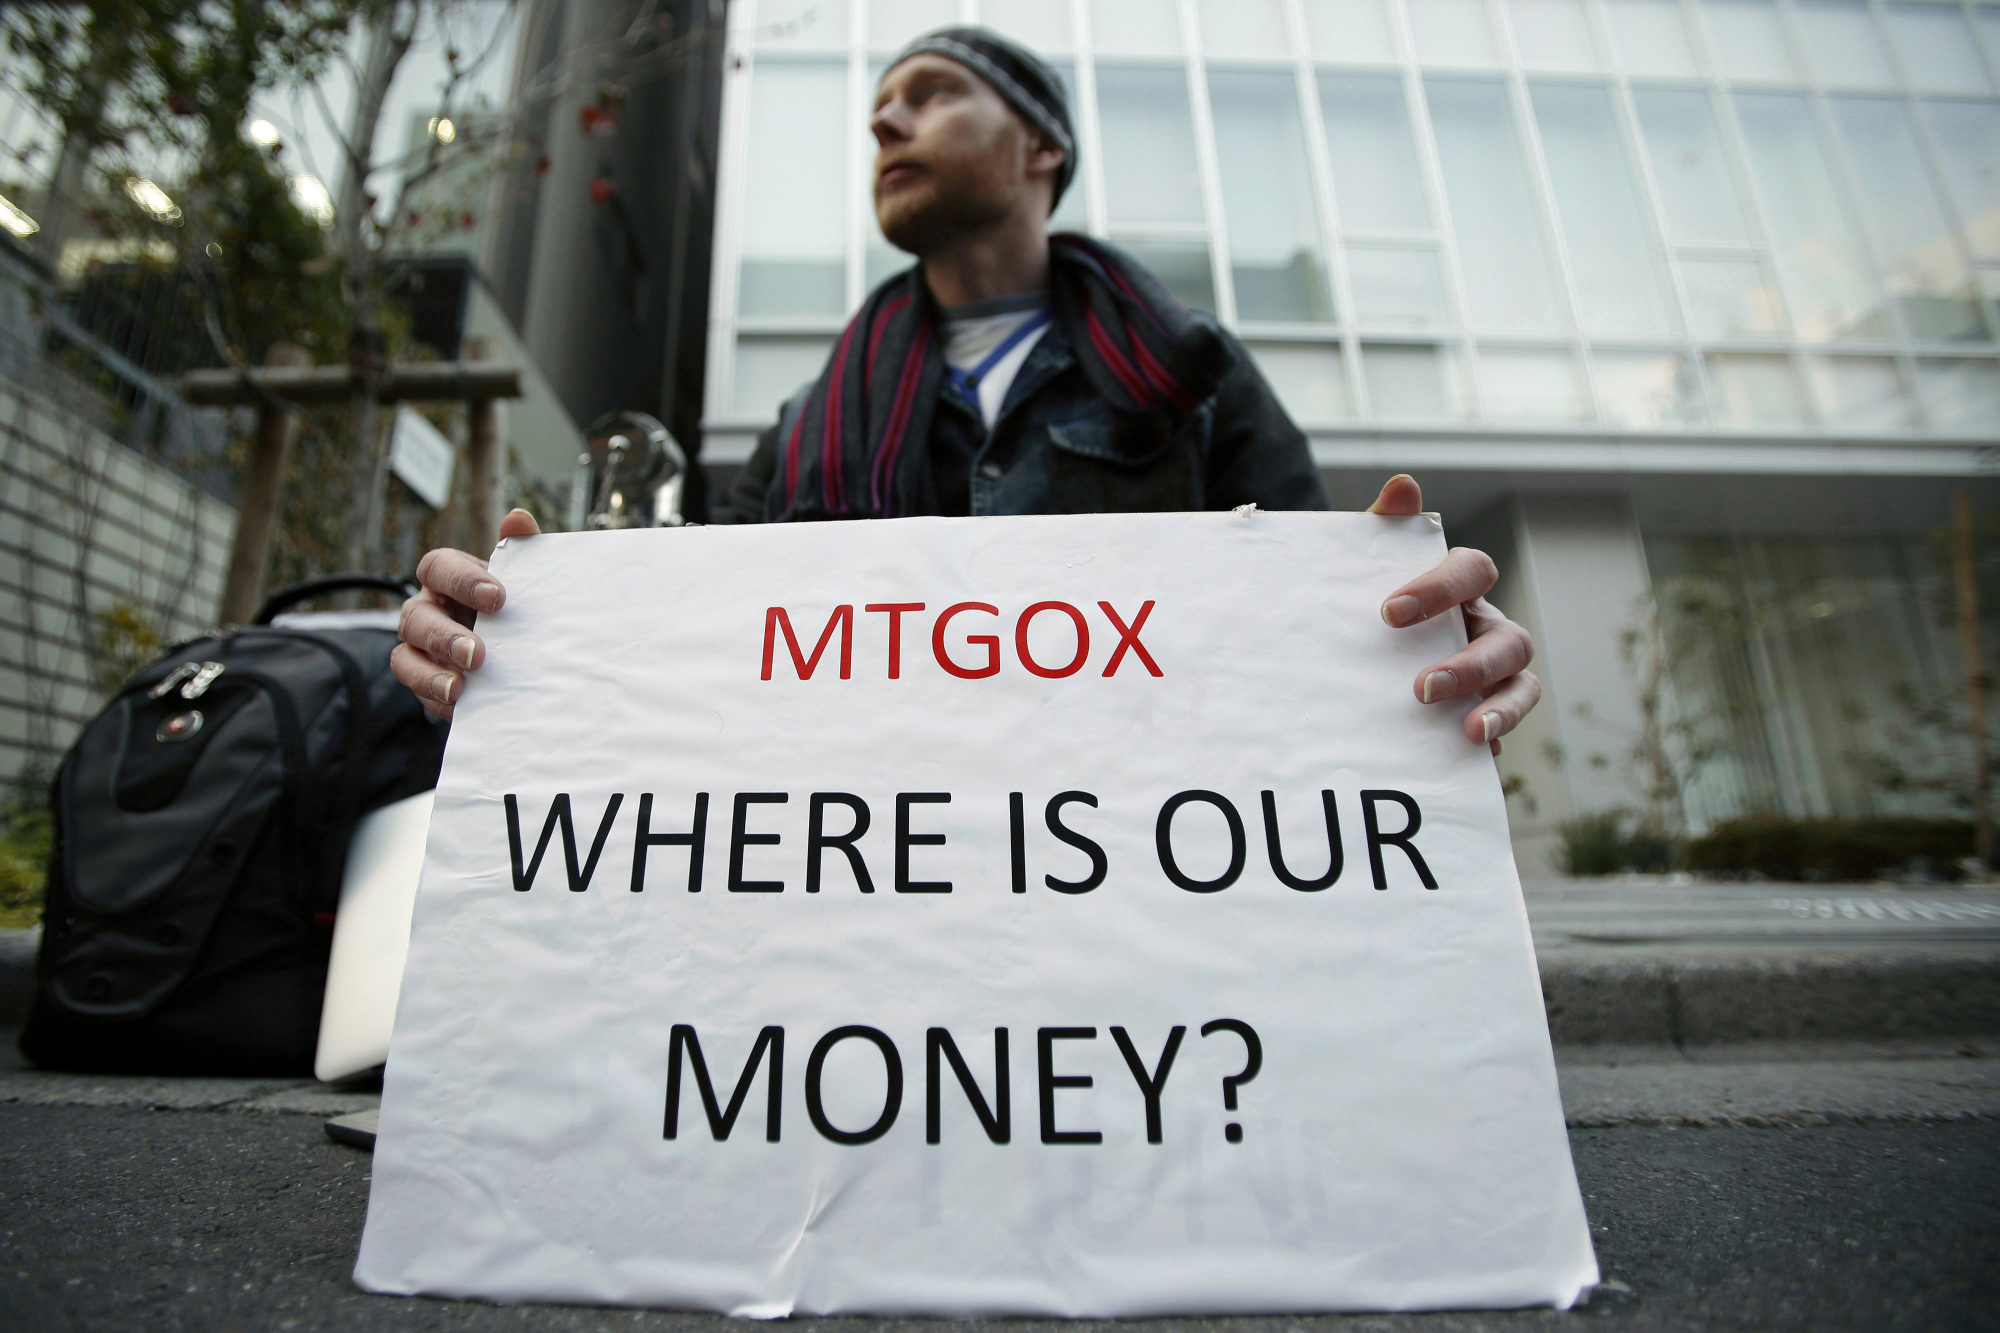
\includegraphics[width=4.6cm]{mtgox.jpg}
  \caption*{[6]}
\end{figure}

\newpage
\section{BITCOIN ECONOMY}
If the government doesn't regulate or control Bitcoin, then who does? How Bitcoin's economy is determined is solely based on the people. "Bitcoin is a monopoly run by a protocol, not by a managing organization"\textbf{[7]}. This means that unlike a traditional monopoly where a corporation is dominate in the economy, in Bitcoin, the process is what has power over the monopoly. The process of consumers making transactions, miners getting transaction fees as a reward where the cost determines how much the person wants to expedite their transaction, and exchanges being brokers to consumers as well. Although people enjoy their privacy when using cryptocurrency and like that the government has no power over it, there are some downsides to no government intervention that can effect the economy of Bitcoin as well. There is the security issues that people must sacrifice for their privacy. If hackers get a hold of credentials, there could be another incident where consumers are losing millions worth of Bitcoin and will even alter the economy of it. Whatever is lost cannot be reversed and users that lose access to their accounts cannot regain access to it once more which makes it a risky gamble for those that do partake in exchanging. Bitcoin's economy is considered revolutionary and interesting to study due to how complex and different it is from our normal market. This is where miners, the people, have full control of the monopoly of Bitcoin. 
\begin{figure}[h!]
  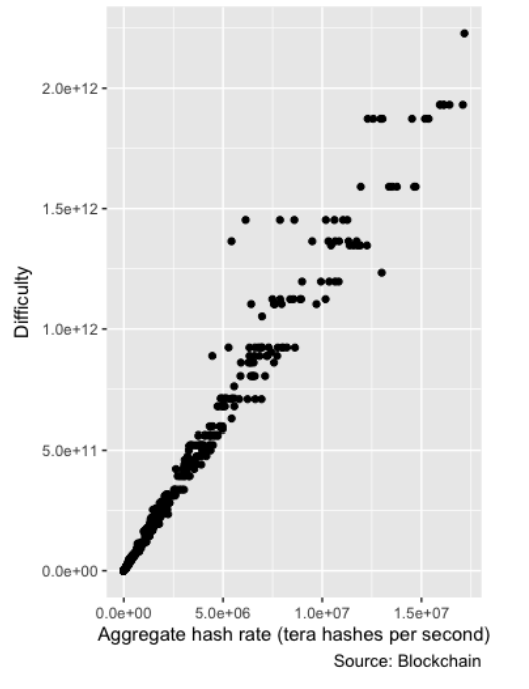
\includegraphics[width=8cm]{ye.PNG}
  \caption*{[8]}
\end{figure}
\begin{figure}[h!]
  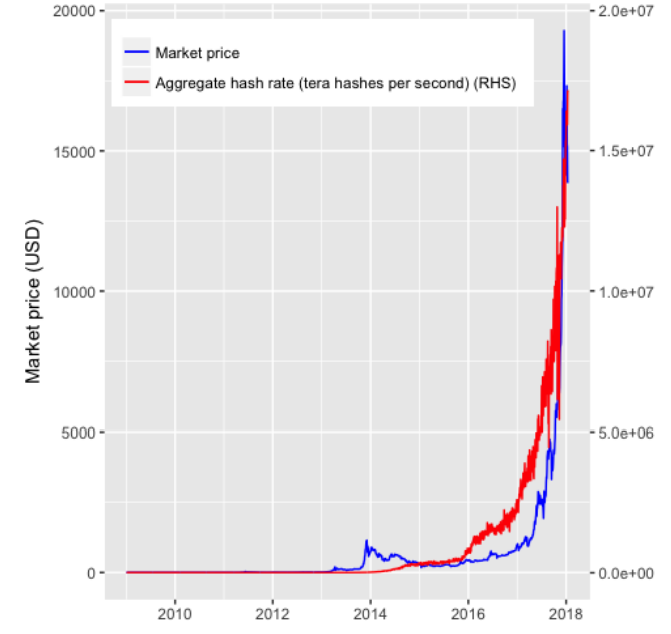
\includegraphics[width=8cm]{market.PNG}
  \caption*{[9]}
\end{figure}
\begin{figure}[h!]
  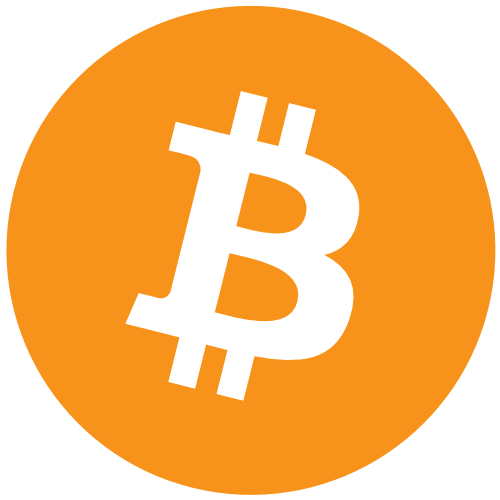
\includegraphics[width=2cm]{bit.png}
  \caption*{[10]}
\end{figure}


\begin{thebibliography}{99}

\bibitem{c1} Conway, L. (2020, November 17). Blockchain Explained. Retrieved May 11, 2021, from https://www.investopedia.com/terms/b/blockchain.asp\&nbsp;
\bibitem{c2}Khairuddin, I. E., \&amp; Sas, C. (2019, May). An Exploration of Bitcoin Mining Practices: Miners' Trust Challenges and Motivations. Retrieved May 11, 2021, from https://dl-acm-org.arcadia.idm.oclc.org/doi/10.1145/3290605.3300859
\bibitem{c3} Nofer, M., Gomber, P., Hinz, O., \&amp; Schiereck, D. (2017, January 20). Blockchain. Retrieved May 11, 2021, from https://www.researchgate.net/publication/315462390\_Blockchain


\bibitem{c4}Li, X., Jiang, P., Chen, T., Luo, X., \&amp; Wen, Q. (2017, August 23). A survey on the security of blockchain systems. Retrieved May 11, 2021, from https://www.sciencedirect.com/science/article/pii/S0167739X17318332

\bibitem{c5} Ma, J., Gans, J. S., \&amp; Tourky, R. (2018, January). Market Structure in Bitcoin Mining. Retrieved May 11, 2021, from https://www.nber.org/system/files/working\_papers/w24242/w24242.pdf

\bibitem{c6} Harney, A., \&amp; Stecklow, S. (2017, November 30). Bitcoin's surge little comfort for burned Mt. GOX clients in international legal limbo. Retrieved May 11, 2021, from https://www.japantimes.co.jp/news/2017/11/30/national/crime-legal/bitcoins-surge-little-comfort-burned-mt-gox-clients-international-legal-limbo/
\bibitem{c7} Huberman, G., Leshno, J., \&amp; Moallemi, C. (2017, September 06). Monopoly without a monopolist: An economic analysis of the bitcoin payment system. Retrieved May 11, 2021, from https://papers.ssrn.com/sol3/papers.cfm?abstract\_id=3032375
\bibitem{c8} Huberman, G., Leshno, J., \&amp; Moallemi, C. (2017, September 06). Monopoly without a monopolist: An economic analysis of the bitcoin payment system. Retrieved May 11, 2021, from https://papers.ssrn.com/sol3/papers.cfm?abstract\_id=3032375
\bibitem{c9} Huberman, G., Leshno, J., \&amp; Moallemi, C. (2017, September 06). Monopoly without a monopolist: An economic analysis of the bitcoin payment system. Retrieved May 11, 2021, from https://papers.ssrn.com/sol3/papers.cfm?abstract\_id=3032375
\bibitem{c10} B. (2009). Open source p2p money. Retrieved May 12, 2021, from https://bitcoin.org/en/



\end{thebibliography}




\end{document}
